\documentclass[11pt]{article}
\usepackage[utf8]{inputenc}
\usepackage{amsmath}
\usepackage{amssymb,amsfonts,latexsym,cancel}
\usepackage{graphicx}
\usepackage{verbatim}
\usepackage{epstopdf}
\usepackage{tabularx} 
\usepackage{float}
\usepackage[left=2cm, right=2cm, top=2cm, bottom=2cm]{geometry}
\setlength\parindent{0pt}
\setlength{\parskip}{2mm}

\title{MultiFEBE \\ME-ST-SR-003 [TUTORIAL] \\ \textbf{Scordelis-Lo Roof (FEM model)}}
\author{Samuel González-Jiménez and Jacob D. R. Bordón}
\date{September 2025}

\begin{document}
	\maketitle
	
	\section*{Problem description}
	In this validation case a static analysis of the Scordelis-Lo roof problem~\cite{MacNeal1985} is performed using the Finite Element method. As shown in Figure \ref{Scord_draw} the problem consist on a curved roof with a 25.0 in radio a 50.0 in length and a thickness of 0.25 in. The properties of the material are a Young modulus (E) of $4.32 \times 10^{8}   \ \text{lbf}/\text{in}^2$ and a Poisson ratio ($\nu$) of 0.0. The roof is under a uniform pressure of $90.0 \ \text{lbf}/\text{in}^2$ in -Z direction. The boundary supports conditions are $u_x = u_z = 0$ on curved edges. The mesh is $N \times N$ on shaded area.
	
	
	\begin{figure}[H]
		\centering
		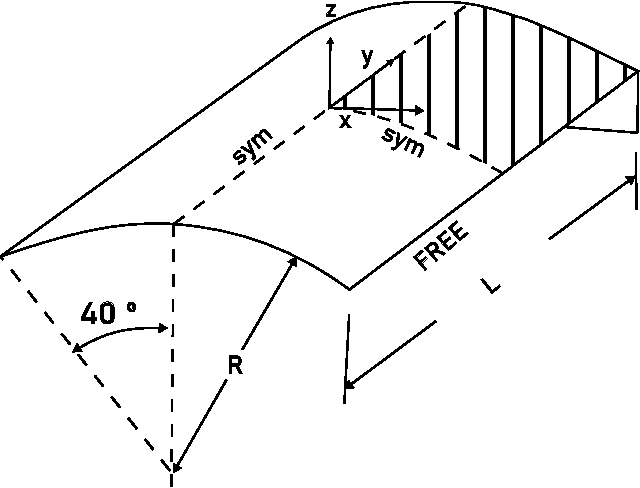
\includegraphics[scale=0.60]{Scordelis_draw.pdf}
		\caption{Scordelis-Lo roof problem}
		\label{Scord_draw}
	\end{figure}
		
	
	\section*{Input data file}
	In this section, the principal block sections of the MultiFEBE input data file will be reviewed.
	The first block to be dealt is the settings one. In this case the mesh is imported from another file named \texttt{"cylindrical\_shell.msh"} in the Gmsh MSH format version 2.2.
	
	\begin{verbatim}
	[settings]
	mesh\_file_mode = 2 "cylindrical_shell.msh"
	\end{verbatim}
		
	In the section [symmetry], two planes of symmetry are defined, since only a quarter of the roof is meshed as shown in Figure \ref{Scord_draw}. To the correct recognition of the symmetry planes, each axis of symmetry must intersect the origin of coordinates.
		
	\begin{verbatim}
	[symmetry planes]
	plane_n1: symmetry
	plane_n2: symmetry
	\end{verbatim}
				
	Since the problem is solved with Shell finite elements, in the [cross sections] section are defined
	the number of fe subregions related to the cross section (1), fe subregion identifier (1), type of
	cross section (degshell), thickness (0.25) and reference vector for x' direction (0. 1. 0.).
	
	\begin{verbatim}
	[cross sections]
	1
	degshell 1 1 0.25 0. 1. 0.
	\end{verbatim}
		
	In the [groups] section, 3 groups are defined. The group 1 selects all the nodes of the XZ plane at y=25, where the boundary support condition will be defined. The group 2 and 3 are composed by all the elements and nodes respectively.
	
	\begin{verbatim}
	[groups]
	3
	1 nodes box interior -100.d0 100.d0 24.99d0 25.01d0 -100.d0 100.d0 1
	2 elements all
	3 nodes all
	\end{verbatim}
	
	In the [fem node options], it is defined that all the nodes results are displayed with 6 degrees of freedom instead of 5 as established by default for shell elements.	
	
	\begin{verbatim}
	[fem node options]
	group 3 n_dof 6}
	\end{verbatim}
	In [conditions over nodes] section, the boundary support is defined.
	\begin{verbatim}
	[conditions over nodes]
	group 1: 0 0.
	         1 0.
	         0 0.
	         1 0.
	         0 0.
	         1 0.
	\end{verbatim}
	
	Finally in [conditions over fe elements] all the elements are loaded with the uniform pressure.
	\begin{verbatim}
	[conditions over fe elements]
	group 2: global
	         1 0. 0.d0 0.d0 -90.d0
	\end{verbatim}
	\section*{Results and discussion}
	
	In this section the results for the convergence of an NxN study is shown. In total 20 meshes were tested, with 2, 4, 8 and 16 elements and 5 different types of elements, i.e. MITC3i, MITC6a, MITC8* and MITC9 (see~\cite{Bathe2006}). The characteristics of each type of element is shown in Table \ref{MITC_tab}.
	
	\begin{table}[H]
	\caption{Element types characteristics}
	\label{MITC_tab}
	\centering
	\begin{tabular}{|c|c|c|}
		\hline
		\textbf{Element} & \textbf{Element shape} & \textbf{Order} \\
		\hline
		MITC3i & Triangular & Linear \\
		\hline
		MITC6a & Triangular & Quadratic \\
		\hline
		MITC4 & Quadrilateral & Linear \\
		\hline
		MITC8* & Quadrilateral & Quadratic \\
		\hline
		MITC9 & Quadrilateral & Quadratic \\
		\hline
	\end{tabular}
\end{table}
	
	Figure \ref{midside} shows the convergence to the mid-side vertical displacement to the theoretical result of 0.3024 in for each element type according to the number of elements.
	
	\begin{figure}[H]
		\centering
		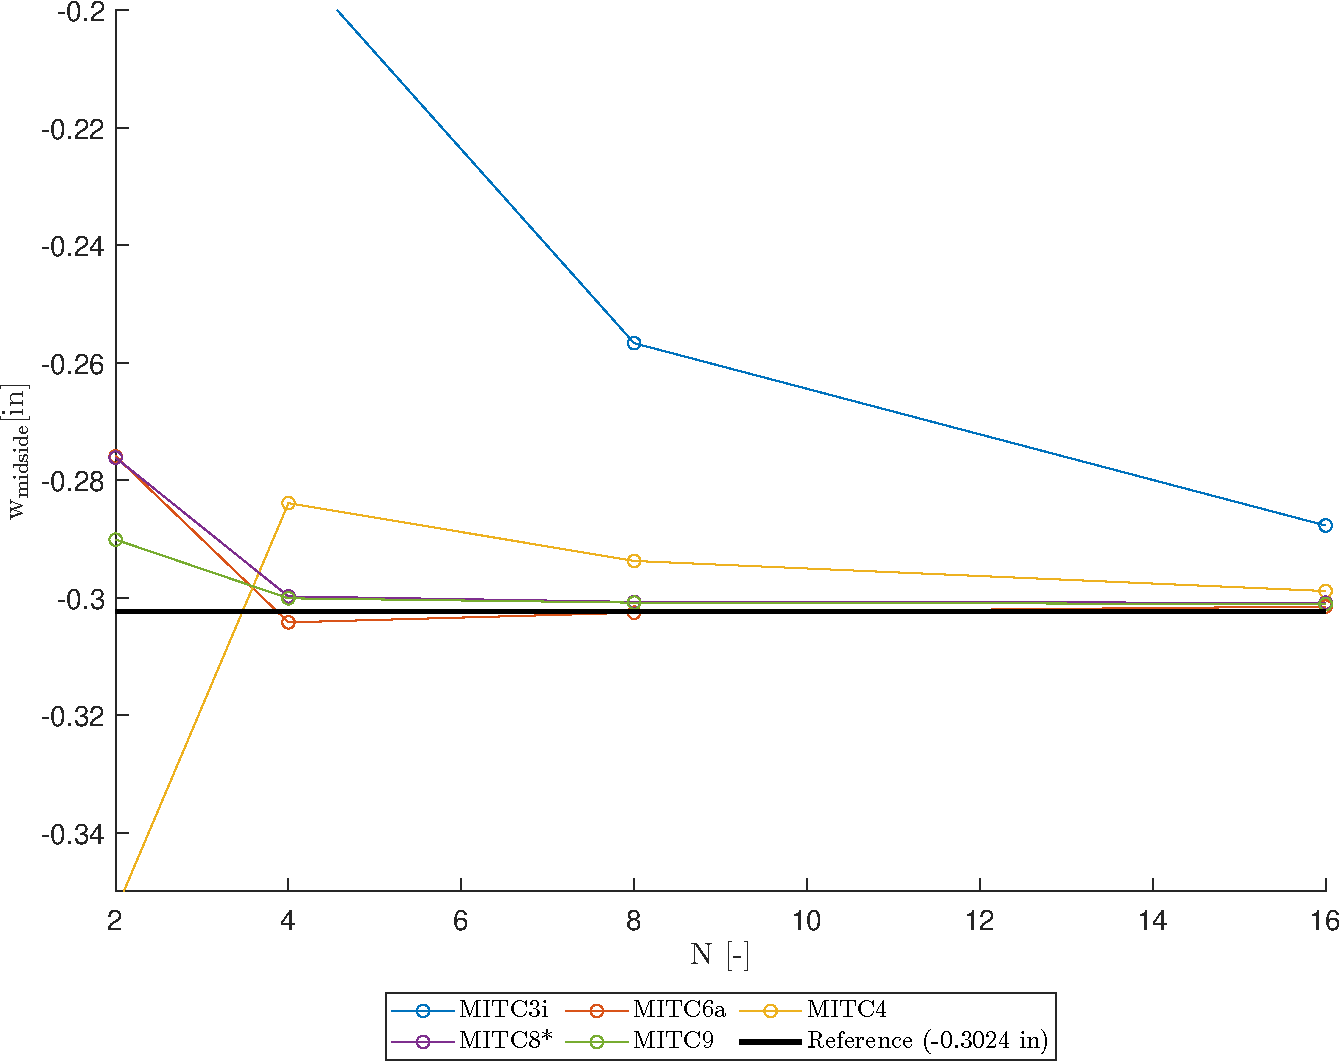
\includegraphics[scale=0.55]{w_midside.pdf}
		\caption{Mid-side vertical displacement convergence study.}
		\label{midside}
	\end{figure}
	
	In Figures \ref{MITC3i}, \ref{MITC4}, \ref{MITC6a}, \ref{MITC8} and \ref{MITC9} the vertical displacement, Nx, My and Qy in the XZ symmetry plane is shown as a function of the curvature angle, as presented in~\cite{Oñate2013}.
	
	\begin{figure}[H]
		\centering
		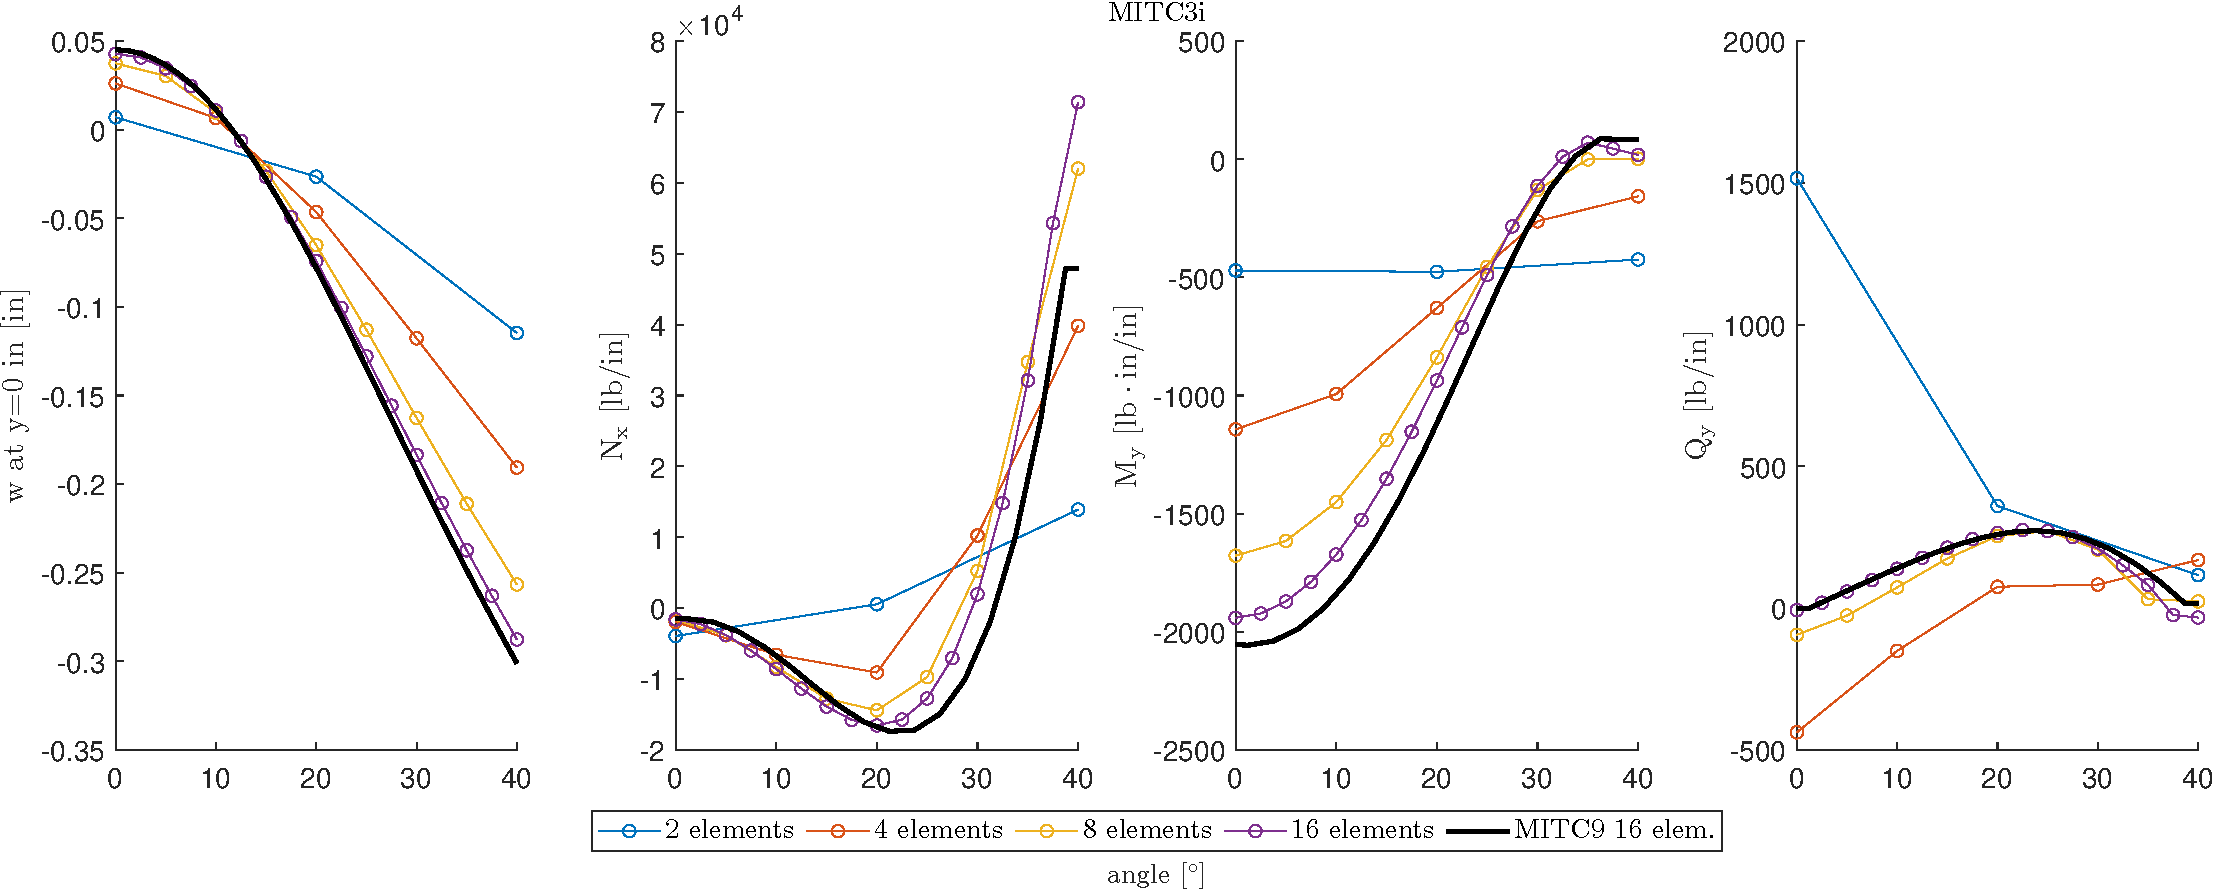
\includegraphics[scale=0.45]{stress_resultants_&_deformed_shape_MITC3i.pdf}
		\caption{Convergence study result for MITC3i elements case.}
		\label{MITC3i}
	\end{figure}
	
		\begin{figure}[H]
		\centering
		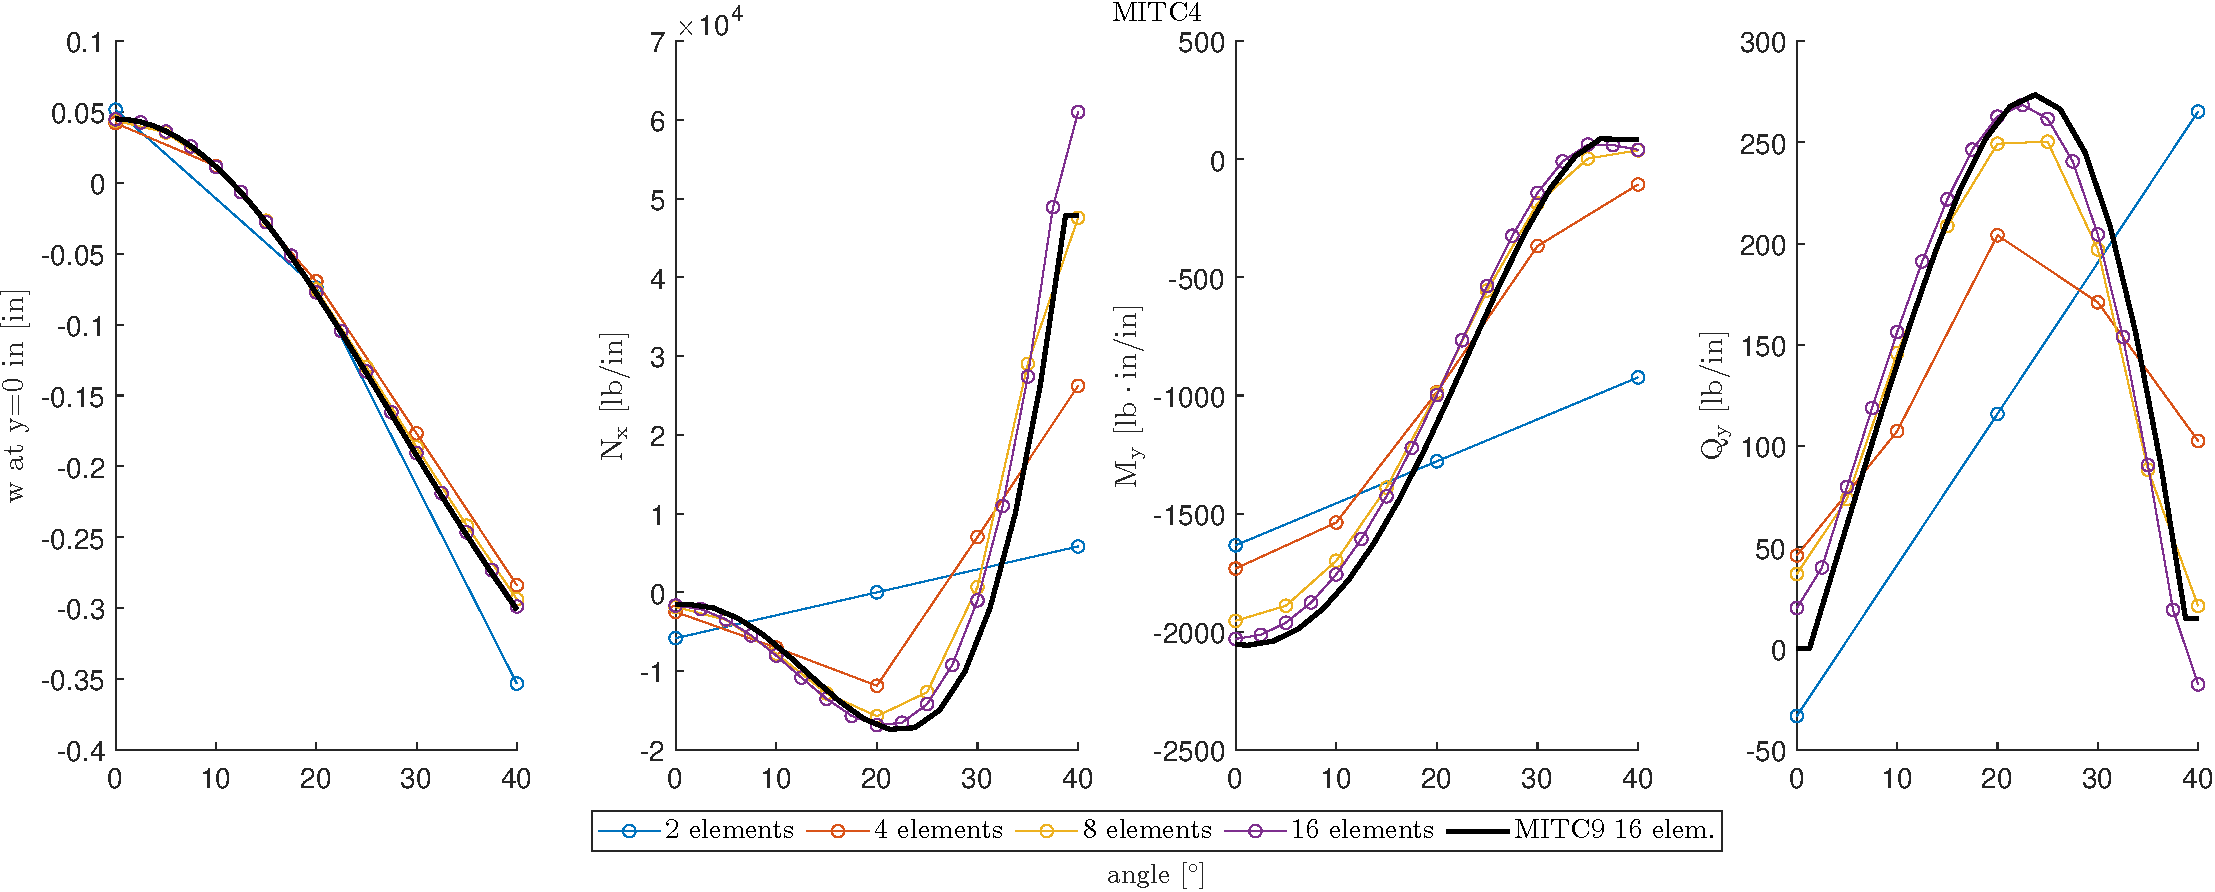
\includegraphics[scale=0.45]{stress_resultants_&_deformed_shape_MITC4.pdf}
		\caption{Convergence study result for MITC4 elements case.}
		\label{MITC4}
	\end{figure}
	
		\begin{figure}[H]
		\centering
		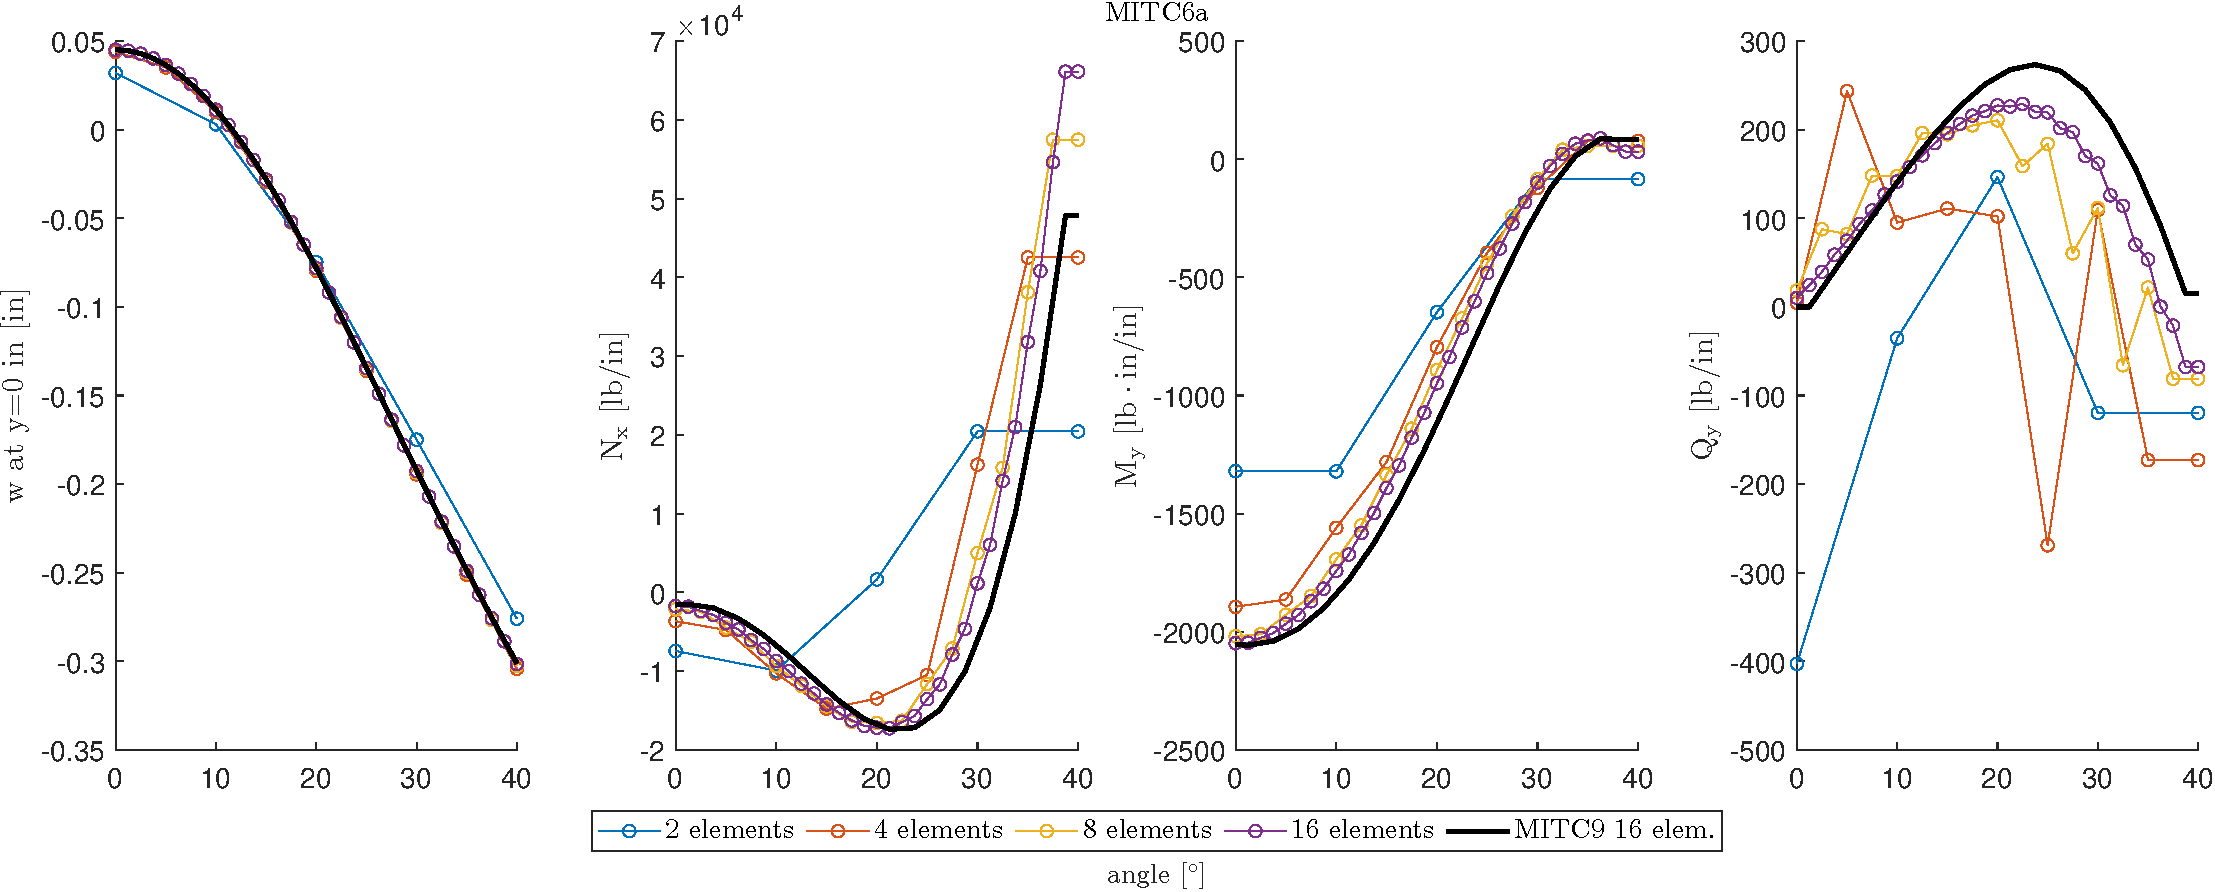
\includegraphics[scale=0.45]{stress_resultants_&_deformed_shape_MITC6a.pdf}
		\caption{Convergence study result for MITC6a elements case.}
		\label{MITC6a}
	\end{figure}
	
		\begin{figure}[H]
		\centering
		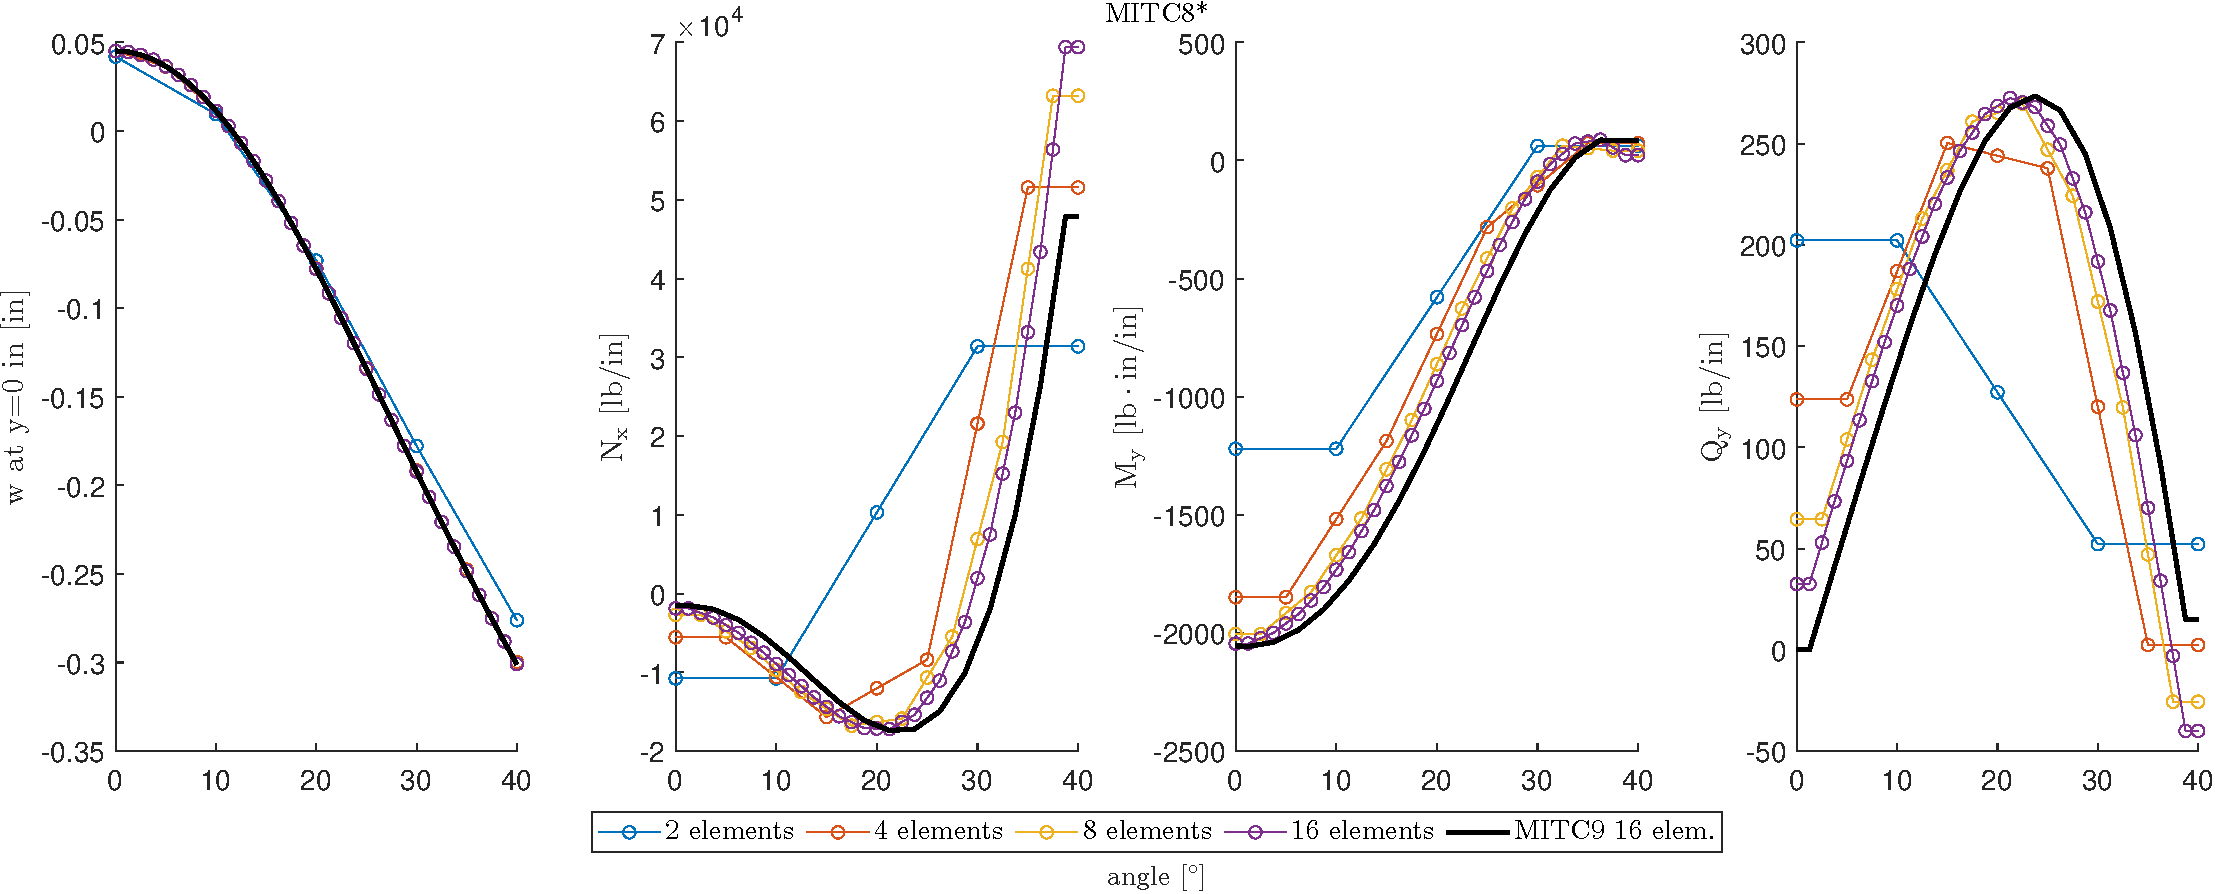
\includegraphics[scale=0.45]{stress_resultants_&_deformed_shape_MITC8.pdf}
		\caption{Convergence study result for MITC8* elements case.}
		\label{MITC8}
	\end{figure}
	
		\begin{figure}[H]
		\centering
		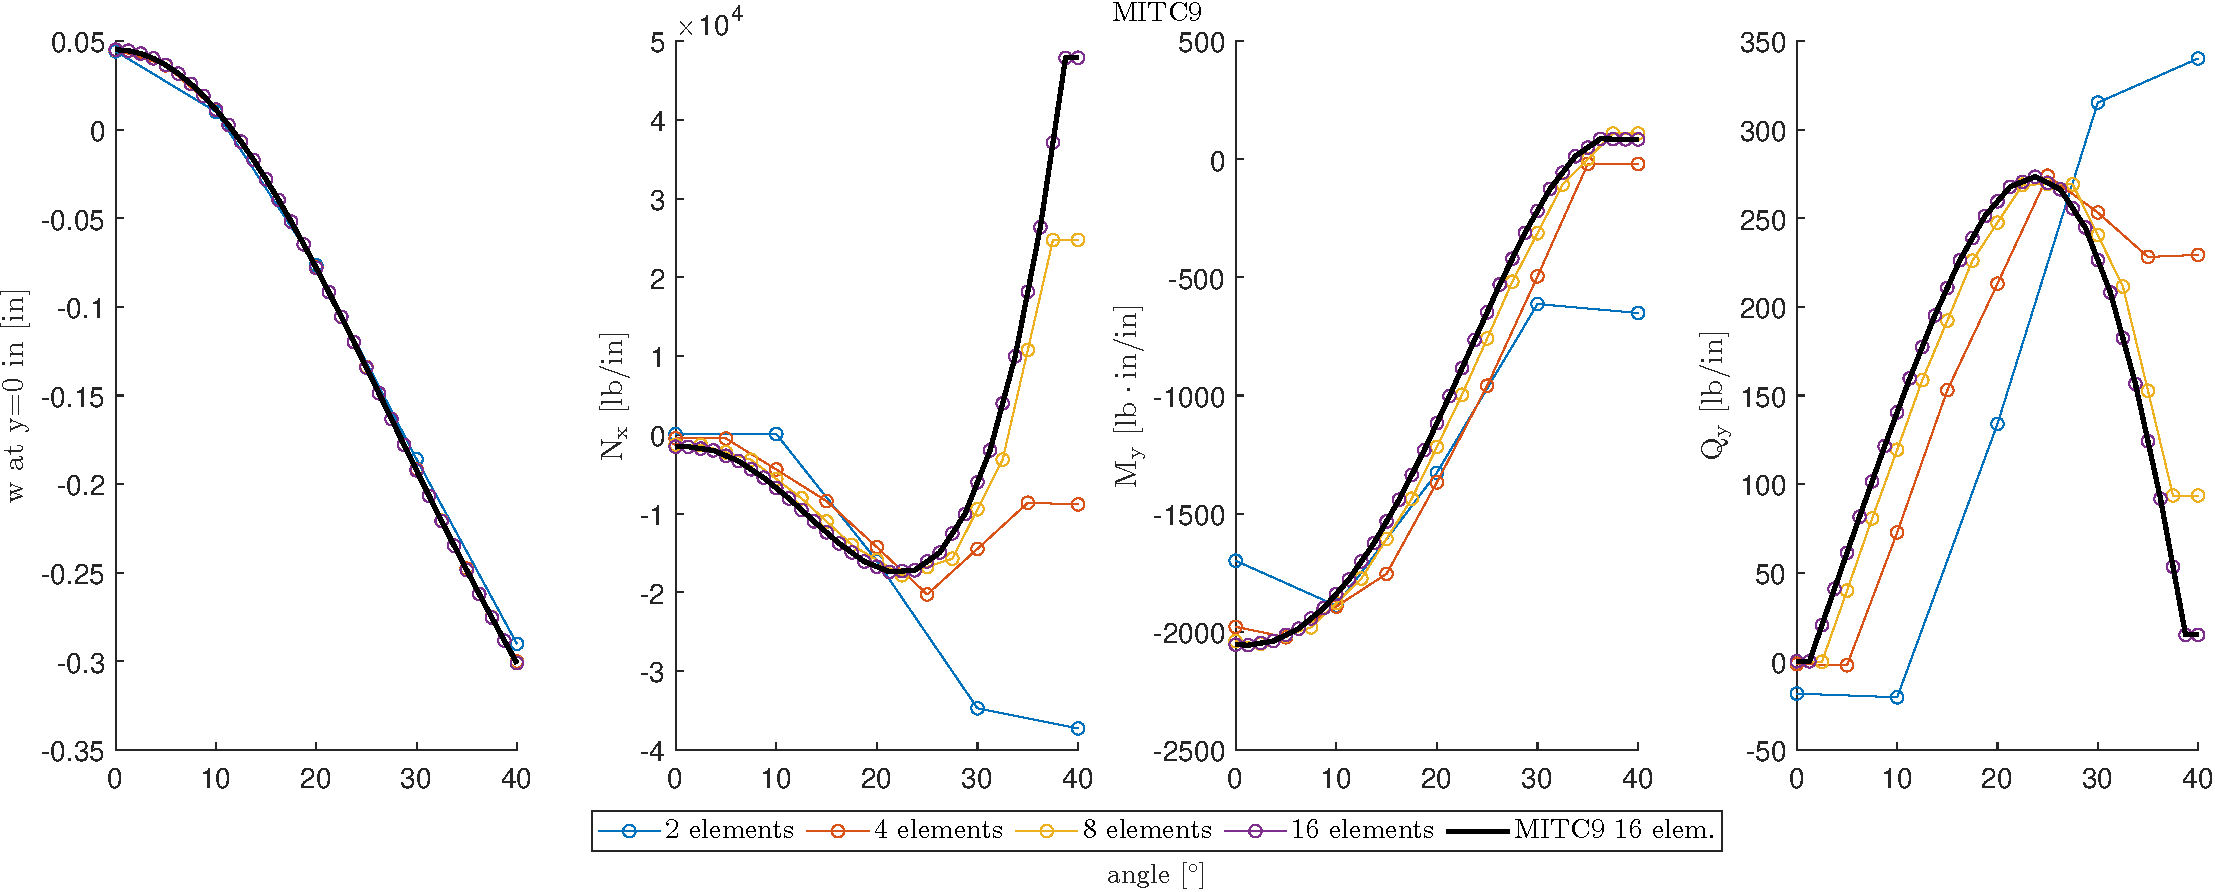
\includegraphics[scale=0.45]{stress_resultants_&_deformed_shape_MITC9.pdf}
		\caption{Convergence study result for MITC9 elements case.}
		\label{MITC9}
	\end{figure}
	
	Except for case MITC3i, convergence is very close to the reference results, with a faster convergence in cases MITC8* and MITC9.
	
	Figure~\ref{deformed_shape} shows the deformed shape of the meshed roof visualized in Gmsh from the .pos file.
	
	\begin{figure}[H]
		\centering
		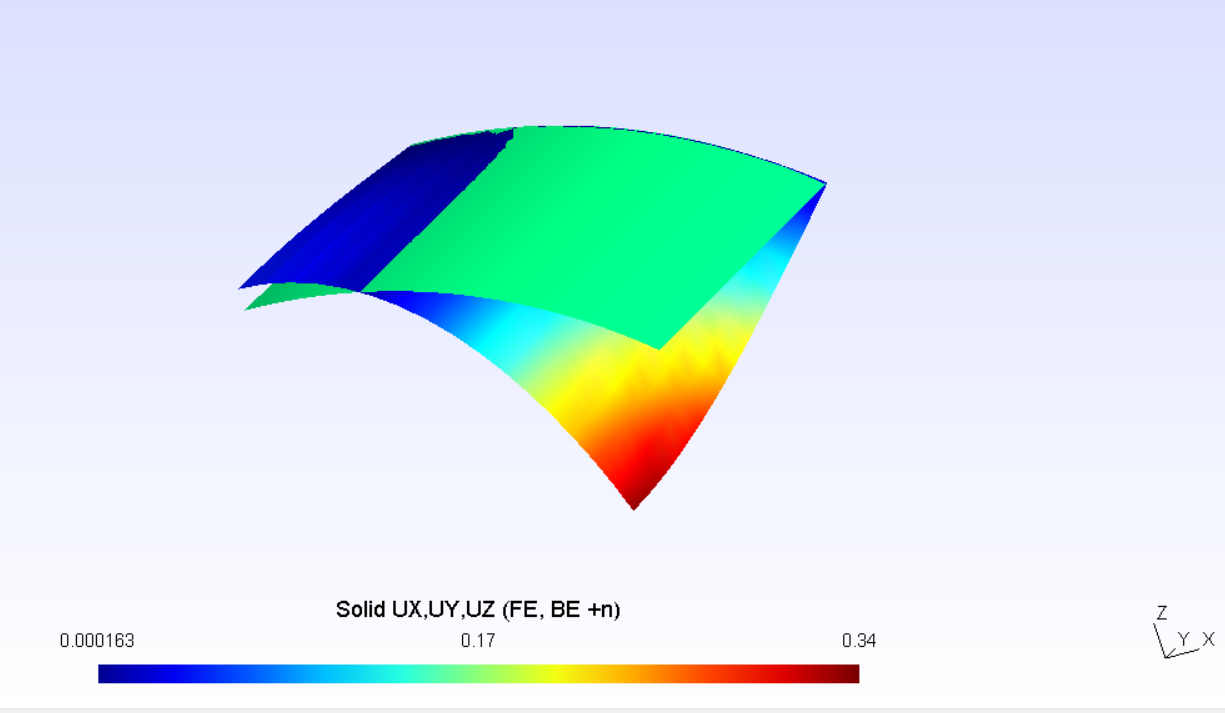
\includegraphics[scale=0.40]{Scordelis-Lo Roof deformed shape}
		\caption{Deformed shape of the quarter of roof for the MITC9 case.}
		\label{deformed_shape}
	\end{figure}
	
	\section*{Attachments}
	 For this validation case, the convergence study execution file is attached as well as the .dat, .mesh and the .geo file. An alternative .dat file without the [symmetry] section, where all the symmetry conditions are defined manually is attached too, which displays the same results as the reviewed one.
	 
	 \bibliographystyle{unsrt}
	 \bibliography{references.bib}
	 
	 \end{document}